\documentclass[12pt]{article}
\pagenumbering{gobble}

\usepackage{amsmath}
\usepackage{amsfonts}
\usepackage{amssymb}
\usepackage{fancyhdr}
\usepackage[headheight=0.25in,margin=1in]{geometry}
\usepackage{makecell}

\usepackage{tikz}
\usetikzlibrary{math}

\tikzstyle{deadline}=[
        draw=red,
        very thick
]

\tikzstyle{running}=[
        fill=blue!25!white
]

\usepackage{pgfplots}
\pgfplotsset{compat=1.18}

\newcommand{\parens}[1]{\ensuremath{
    \left( #1 \right)
}}

\newcommand{\brackets}[1]{\ensuremath{
    \left[ #1 \right]
}}

\newcommand{\N}{\mathbb{N}}
\newcommand{\Z}{\mathbb{Z}}
\newcommand{\Q}{\mathbb{Q}}
\newcommand{\R}{\mathbb{R}}
\newcommand{\C}{\mathbb{C}}

\newcommand{\solution}{\textbf{Solution:}}
\newcommand{\proof}{\textbf{Proof:}}
\newcommand{\done}{\ensuremath{
    \strut\hfill\blacksquare
}}

\linespread{1.25}

\begin{document}
    \pagestyle{fancy}

    \fancyhead[L]{Operating Systems}
    \fancyhead[C]{Assignment 2}
    \fancyhead[R]{Alex Agruso}

    \begin{itemize}
        \item [1.)] \begin{itemize}
            \item [a.)] First Come First Served
                \begin{center}
                    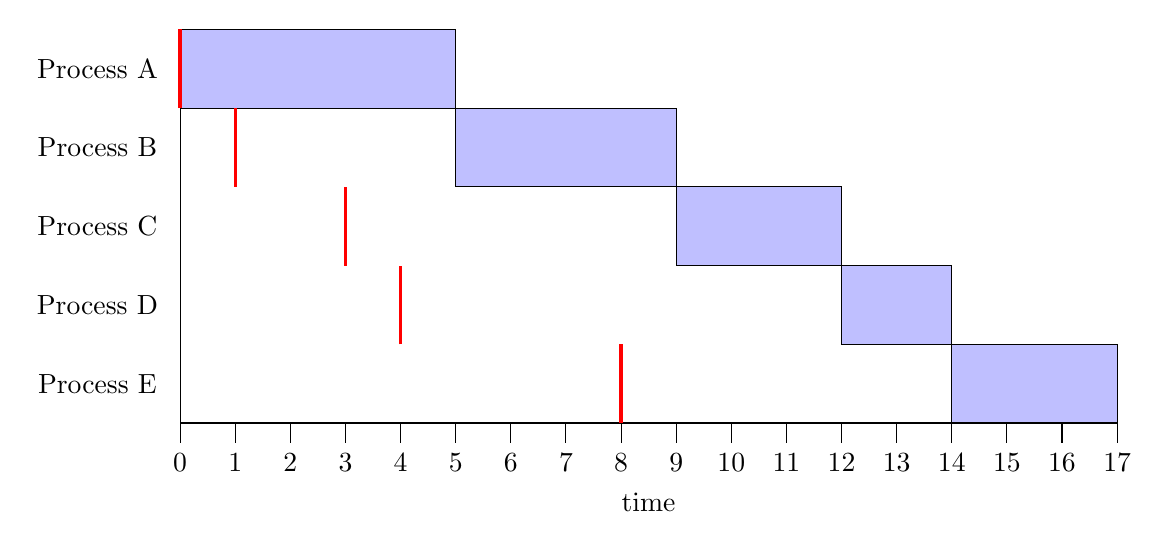
\begin{tikzpicture}[xscale=0.7]
                        \node at (-1.5,4.5) {Process A};
                        \node at (-1.5,3.5) {Process B};
                        \node at (-1.5,2.5) {Process C};
                        \node at (-1.5,1.5) {Process D};
                        \node at (-1.5,0.5) {Process E};
                        \node at (8.5,-1) {time};

                        \draw (0,0) -- (0,5);
                        \draw (0,0) -- (17,0);
                        
                        \pgfkeys{/pgf/number format/precision=0}

                        \foreach \i in {0,...,17} {
                            \draw (\i,0) -- (\i,-0.25);
                            \node at (\i,-0.5) {\i};
                        }

                        \draw[fill=blue!25!white] (0,4) rectangle (5,5);
                        \draw[fill=blue!25!white] (5,3) rectangle (9,4);
                        \draw[fill=blue!25!white] (9,2) rectangle (12,3);
                        \draw[fill=blue!25!white] (12,1) rectangle (14,2);
                        \draw[fill=blue!25!white] (14,0) rectangle (17,1);

                        \draw[deadline] (0,4) -- (0,5);
                        \draw[deadline] (1,3) -- (1,4);
                        \draw[deadline] (3,2) -- (3,3);
                        \draw[deadline] (4,1) -- (4,2);
                        \draw[deadline] (8,0) -- (8,1);
                        
                    \end{tikzpicture}
                \end{center}

                \begin{tabular}{llllll}
                    A & B & C & D & E \\
                    \hline
                    5 & 9 & 12 & 14 & 17
                    & \makecell{completion time}
                \end{tabular}

                Average Turnaround: 8.2

                Average Normalized Turnaround: 2.8

            \item [b.)] Round Robin \( (q = 1) \)
                \begin{center}
                    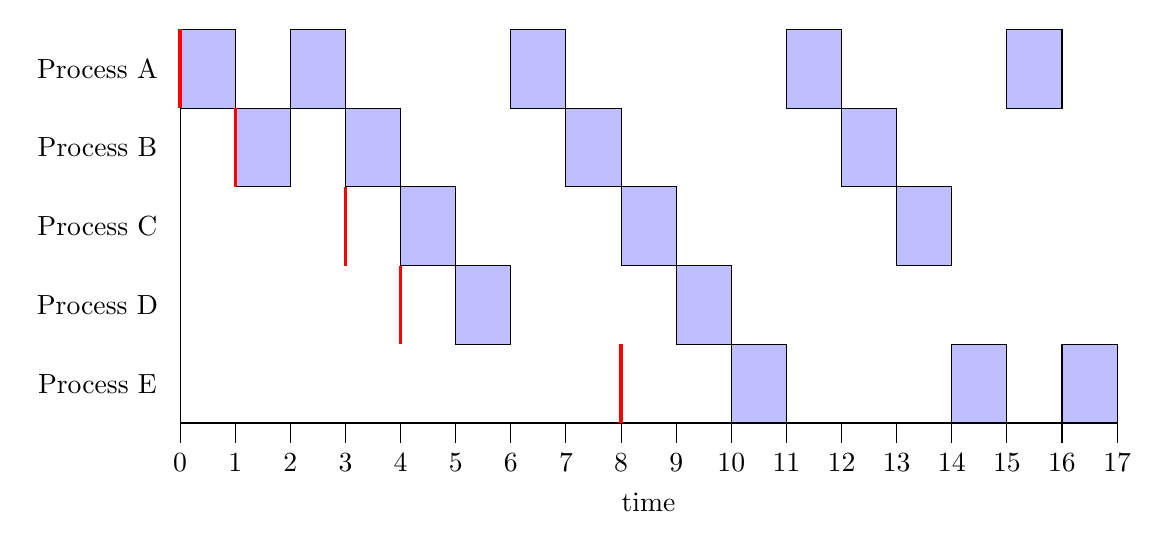
\begin{tikzpicture}[xscale=0.7]
                        \node at (-1.5,4.5) {Process A};
                        \node at (-1.5,3.5) {Process B};
                        \node at (-1.5,2.5) {Process C};
                        \node at (-1.5,1.5) {Process D};
                        \node at (-1.5,0.5) {Process E};
                        \node at (8.5,-1) {time};

                        \draw (0,0) -- (0,5);
                        \draw (0,0) -- (17,0);
                        
                        \pgfkeys{/pgf/number format/precision=0}

                        \foreach \i in {0,...,17} {
                            \draw (\i,0) -- (\i,-0.25);
                            \node at (\i,-0.5) {\i};
                        }

                        
                        \draw[running] (0,4) rectangle (1,5);
                        \draw[running] (2,4) rectangle (3,5);
                        \draw[running] (6,4) rectangle (7,5);
                        \draw[running] (11,4) rectangle (12,5);
                        \draw[running] (15,4) rectangle (16,5);

                        \draw[running] (1,3) rectangle (2,4);
                        \draw[running] (3,3) rectangle (4,4);
                        \draw[running] (7,3) rectangle (8,4);
                        \draw[running] (12,3) rectangle (13,4);

                        \draw[running] (4,2) rectangle (5,3);
                        \draw[running] (8,2) rectangle (9,3);
                        \draw[running] (13,2) rectangle (14,3);

                        \draw[running] (5,1) rectangle (6,2);
                        \draw[running] (9,1) rectangle (10,2);

                        \draw[running] (10,0) rectangle (11,1);
                        \draw[running] (14,0) rectangle (15,1);
                        \draw[running] (16,0) rectangle (17,1);

                        \draw[deadline] (0,4) -- (0,5);
                        \draw[deadline] (1,3) -- (1,4);
                        \draw[deadline] (3,2) -- (3,3);
                        \draw[deadline] (4,1) -- (4,2);
                        \draw[deadline] (8,0) -- (8,1);
                        
                    \end{tikzpicture}
                \end{center}

                \begin{tabular}{llllll}
                    A & B & C & D & E \\
                    \hline
                    16 & 13 & 14 & 10 & 17
                    & \makecell{completion time}
                \end{tabular}

                Average Turnaround: 10.8

                Average Normalized Turnaround: 3.173

            \pagebreak
            \item [c.)] Round Robin \( (q = 2) \)
                \begin{center}
                    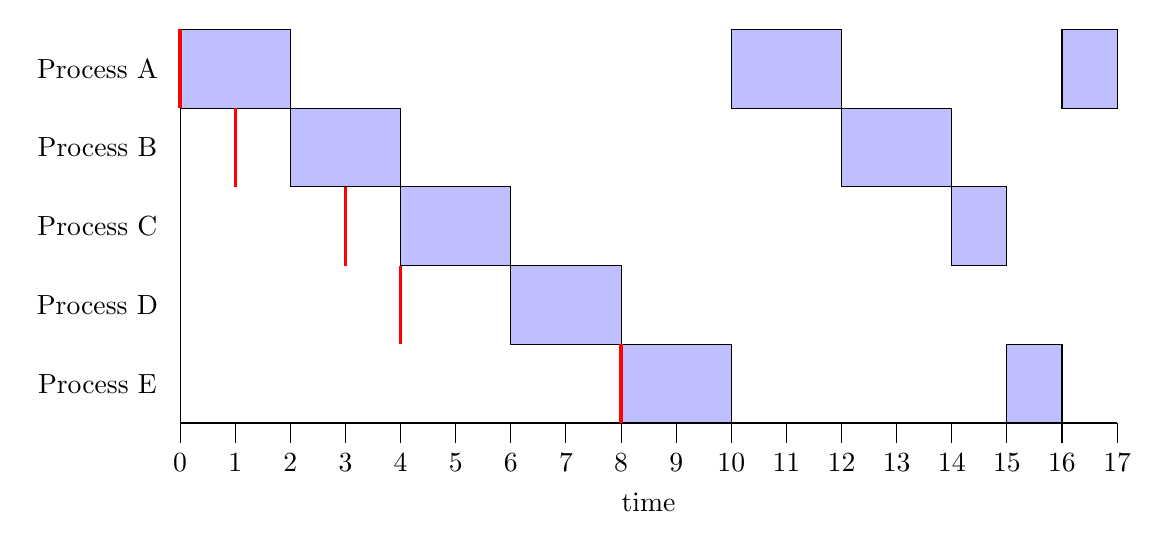
\begin{tikzpicture}[xscale=0.7]
                        \node at (-1.5,4.5) {Process A};
                        \node at (-1.5,3.5) {Process B};
                        \node at (-1.5,2.5) {Process C};
                        \node at (-1.5,1.5) {Process D};
                        \node at (-1.5,0.5) {Process E};
                        \node at (8.5,-1) {time};

                        \draw (0,0) -- (0,5);
                        \draw (0,0) -- (17,0);

                        \foreach \i in {0,...,17} {
                            \draw (\i,0) -- (\i,-0.25);
                            \node at (\i,-0.5) {\i};
                        }

                        
                        \draw[running] (0,4) rectangle (2,5);
                        \draw[running] (10,4) rectangle (12,5);
                        \draw[running] (16,4) rectangle (17,5);

                        \draw[running] (2,3) rectangle (4,4);
                        \draw[running] (12,3) rectangle (14,4);

                        \draw[running] (4,2) rectangle (6,3);
                        \draw[running] (14,2) rectangle (15,3);

                        \draw[running] (6,1) rectangle (8,2);

                        \draw[running] (8,0) rectangle (10,1);
                        \draw[running] (15,0) rectangle (16,1);

                        \draw[deadline] (0,4) -- (0,5);
                        \draw[deadline] (1,3) -- (1,4);
                        \draw[deadline] (3,2) -- (3,3);
                        \draw[deadline] (4,1) -- (4,2);
                        \draw[deadline] (8,0) -- (8,1);
                        
                    \end{tikzpicture}
                \end{center}

                \begin{tabular}{llllll}
                    A & B & C & D & E \\
                    \hline
                    17 & 14 & 15 & 8 & 16
                    & \makecell{completion time}
                \end{tabular}

                Average Turnaround: 10.8

                Average Normalized Turnaround: 3.063

            \item [d.)] Shortest Job First
                \begin{center}
                    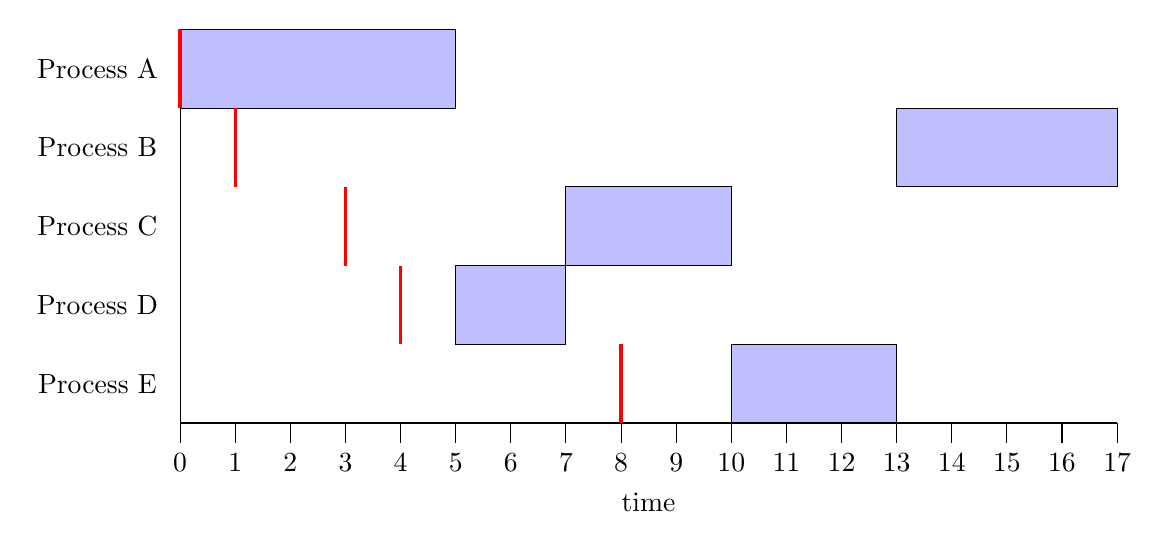
\begin{tikzpicture}[xscale=0.7]
                        \node at (-1.5,4.5) {Process A};
                        \node at (-1.5,3.5) {Process B};
                        \node at (-1.5,2.5) {Process C};
                        \node at (-1.5,1.5) {Process D};
                        \node at (-1.5,0.5) {Process E};
                        \node at (8.5,-1) {time};

                        \draw (0,0) -- (0,5);
                        \draw (0,0) -- (17,0);

                        \foreach \i in {0,...,17} {
                            \draw (\i,0) -- (\i,-0.25);
                            \node at (\i,-0.5) {\i};
                        }

                        \draw[running] (0,4) rectangle (5,5);

                        \draw[running] (13,3) rectangle (17,4);

                        \draw[running] (7,2) rectangle (10,3);

                        \draw[running] (5,1) rectangle (7,2);

                        \draw[running] (10,0) rectangle (13,1);

                        \draw[deadline] (0,4) -- (0,5);
                        \draw[deadline] (1,3) -- (1,4);
                        \draw[deadline] (3,2) -- (3,3);
                        \draw[deadline] (4,1) -- (4,2);
                        \draw[deadline] (8,0) -- (8,1);
                        
                    \end{tikzpicture}
                \end{center}

                \begin{tabular}{llllll}
                    A & B & C & D & E \\
                    \hline
                    5 & 17 & 10 & 7 & 13
                    & \makecell{completion time}
                \end{tabular}

                Average Turnaround: 7.2

                Average Normalized Turnaround: 2.1

            \pagebreak
            \item [e.)] Shortest Remaining Time First
                \begin{center}
                    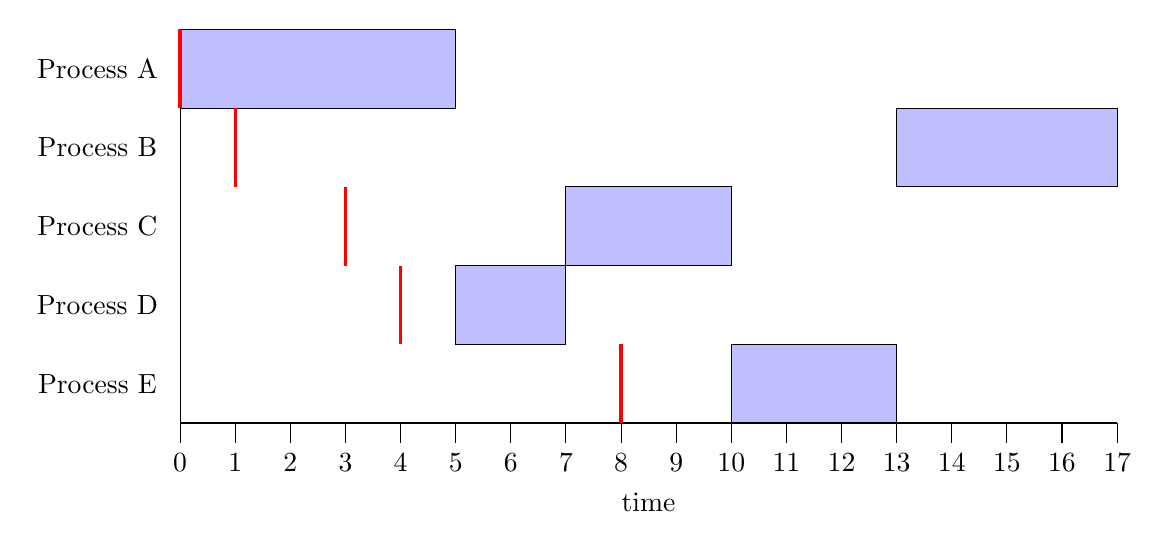
\begin{tikzpicture}[xscale=0.7]
                        \node at (-1.5,4.5) {Process A};
                        \node at (-1.5,3.5) {Process B};
                        \node at (-1.5,2.5) {Process C};
                        \node at (-1.5,1.5) {Process D};
                        \node at (-1.5,0.5) {Process E};
                        \node at (8.5,-1) {time};

                        \draw (0,0) -- (0,5);
                        \draw (0,0) -- (17,0);

                        \foreach \i in {0,...,17} {
                            \draw (\i,0) -- (\i,-0.25);
                            \node at (\i,-0.5) {\i};
                        }

                        \draw[running] (0,4) rectangle (5,5);

                        \draw[running] (13,3) rectangle (17,4);

                        \draw[running] (7,2) rectangle (10,3);

                        \draw[running] (5,1) rectangle (7,2);

                        \draw[running] (10,0) rectangle (13,1);

                        \draw[deadline] (0,4) -- (0,5);
                        \draw[deadline] (1,3) -- (1,4);
                        \draw[deadline] (3,2) -- (3,3);
                        \draw[deadline] (4,1) -- (4,2);
                        \draw[deadline] (8,0) -- (8,1);
                        
                    \end{tikzpicture}
                \end{center}

                \begin{tabular}{llllll}
                    A & B & C & D & E \\
                    \hline
                    5 & 17 & 10 & 7 & 13
                    & \makecell{completion time}
                \end{tabular}

                Average Turnaround: 7.2

                Average Normalized Turnaround: 2.1
            
            \item [f.)] Highest Response Ratio Next
                \begin{center}
                    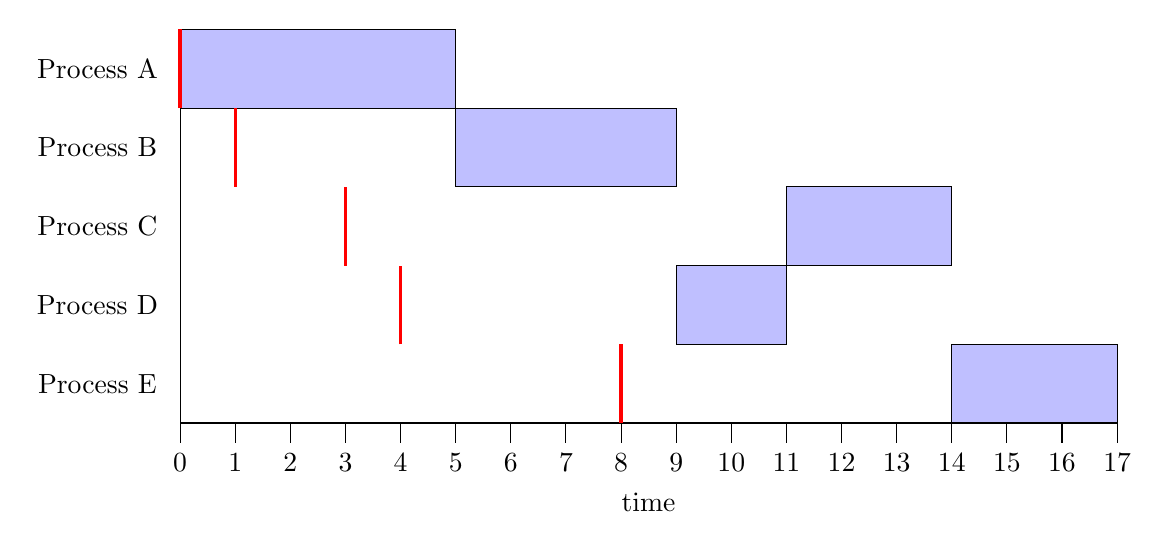
\begin{tikzpicture}[xscale=0.7]
                        \node at (-1.5,4.5) {Process A};
                        \node at (-1.5,3.5) {Process B};
                        \node at (-1.5,2.5) {Process C};
                        \node at (-1.5,1.5) {Process D};
                        \node at (-1.5,0.5) {Process E};
                        \node at (8.5,-1) {time};

                        \draw (0,0) -- (0,5);
                        \draw (0,0) -- (17,0);

                        \foreach \i in {0,...,17} {
                            \draw (\i,0) -- (\i,-0.25);
                            \node at (\i,-0.5) {\i};
                        }

                        \draw[running] (0,4) rectangle (5,5);

                        \draw[running] (5,3) rectangle (9,4);

                        \draw[running] (11,2) rectangle (14,3);

                        \draw[running] (9,1) rectangle (11,2);

                        \draw[running] (14,0) rectangle (17,1);

                        \draw[deadline] (0,4) -- (0,5);
                        \draw[deadline] (1,3) -- (1,4);
                        \draw[deadline] (3,2) -- (3,3);
                        \draw[deadline] (4,1) -- (4,2);
                        \draw[deadline] (8,0) -- (8,1);
                        
                    \end{tikzpicture}
                \end{center}

                \begin{tabular}{llllll}
                    A & B & C & D & E \\
                    \hline
                    5 & 9 & 14 & 11 & 17
                    & \makecell{completion time}
                \end{tabular}

                Average Turnaround: 8

                Average Normalized Turnaround: 2.633

            \pagebreak
            \item [g.)] Multi-level Feedback With 2 Queues
                \begin{center}
                    \text{Queue 1 (First Come First Served, \( q = 1 \))}
                \end{center}
                \begin{center}
                    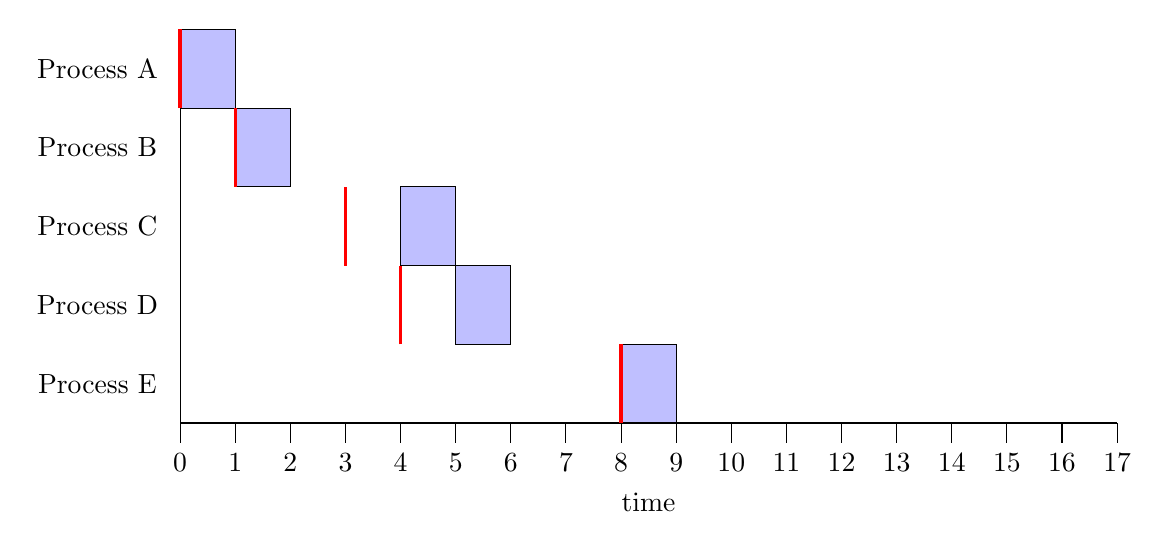
\begin{tikzpicture}[xscale=0.7]
                        \node at (-1.5,4.5) {Process A};
                        \node at (-1.5,3.5) {Process B};
                        \node at (-1.5,2.5) {Process C};
                        \node at (-1.5,1.5) {Process D};
                        \node at (-1.5,0.5) {Process E};
                        \node at (8.5,-1) {time};

                        \draw (0,0) -- (0,5);
                        \draw (0,0) -- (17,0);

                        \foreach \i in {0,...,17} {
                            \draw (\i,0) -- (\i,-0.25);
                            \node at (\i,-0.5) {\i};
                        }

                        \draw[running] (0,4) rectangle (1,5);

                        \draw[running] (1,3) rectangle (2,4);

                        \draw[running] (4,2) rectangle (5,3);

                        \draw[running] (5,1) rectangle (6,2);

                        \draw[running] (8,0) rectangle (9,1);

                        \draw[deadline] (0,4) -- (0,5);
                        \draw[deadline] (1,3) -- (1,4);
                        \draw[deadline] (3,2) -- (3,3);
                        \draw[deadline] (4,1) -- (4,2);
                        \draw[deadline] (8,0) -- (8,1);
                        
                    \end{tikzpicture}
                \end{center}
                \begin{center}
                    \text{Queue 2 (Round Robin, \( q = 2 \))}
                \end{center}
                \begin{center}
                    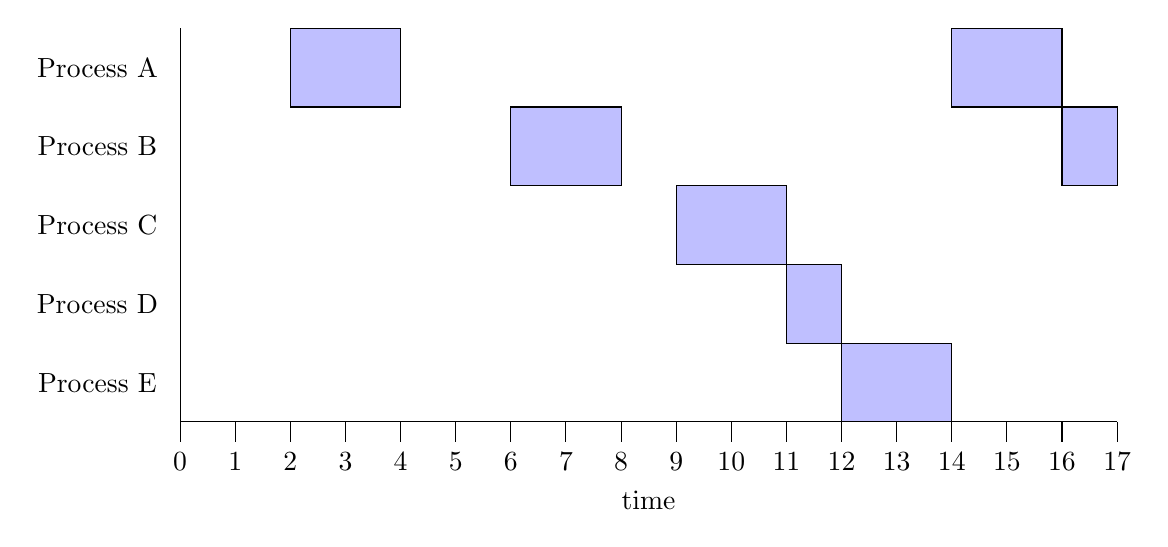
\begin{tikzpicture}[xscale=0.7]
                        \node at (-1.5,4.5) {Process A};
                        \node at (-1.5,3.5) {Process B};
                        \node at (-1.5,2.5) {Process C};
                        \node at (-1.5,1.5) {Process D};
                        \node at (-1.5,0.5) {Process E};
                        \node at (8.5,-1) {time};

                        \draw (0,0) -- (0,5);
                        \draw (0,0) -- (17,0);

                        \draw[running] (2,4) rectangle (4,5);
                        \draw[running] (14,4) rectangle (16,5);

                        \draw[running] (6,3) rectangle (8,4);
                        \draw[running] (16,3) rectangle (17,4);

                        \draw[running] (9,2) rectangle (11,3);

                        \draw[running] (11,1) rectangle (12,2);

                        \draw[running] (12,0) rectangle (14,1);

                        \foreach \i in {0,...,17} {
                            \draw (\i,0) -- (\i,-0.25);
                            \node at (\i,-0.5) {\i};
                        }
                        
                    \end{tikzpicture}
                \end{center}

                \begin{tabular}{llllll}
                    A & B & C & D & E \\
                    \hline
                    16 & 17 & 11 & 12 & 14
                    & \makecell{completion time}
                \end{tabular}

                Average Turnaround: 10.8

                Average Normalized Turnaround: 3.173

           \pagebreak 
            \item [h.)] Preemptive Highest Response Ratio Next \( (q=2) \)
                \begin{center}
                    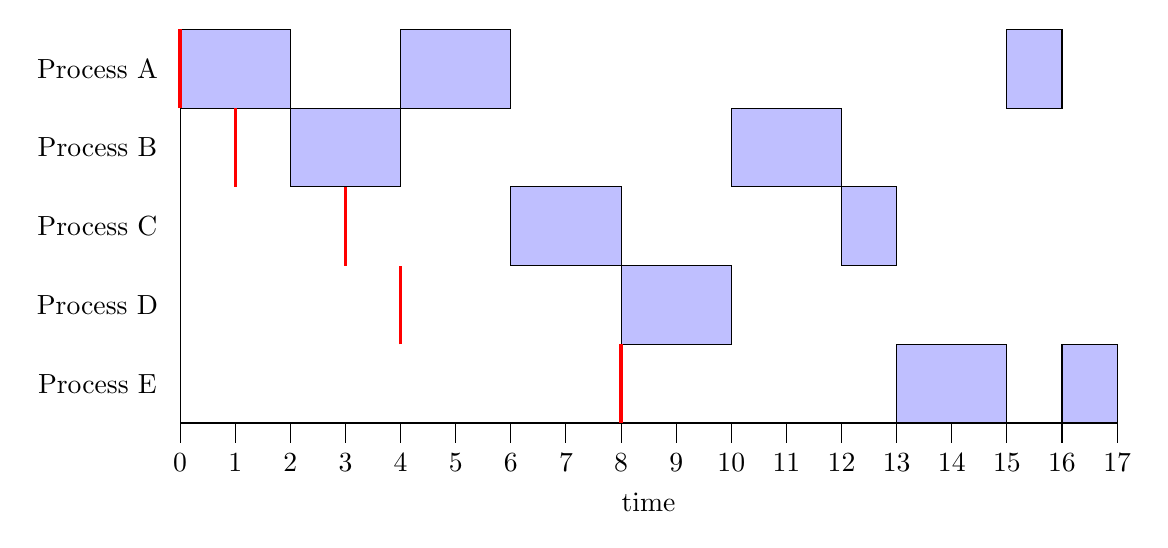
\begin{tikzpicture}[xscale=0.7]
                        \node at (-1.5,4.5) {Process A};
                        \node at (-1.5,3.5) {Process B};
                        \node at (-1.5,2.5) {Process C};
                        \node at (-1.5,1.5) {Process D};
                        \node at (-1.5,0.5) {Process E};
                        \node at (8.5,-1) {time};

                        \draw (0,0) -- (0,5);
                        \draw (0,0) -- (17,0);

                        \foreach \i in {0,...,17} {
                            \draw (\i,0) -- (\i,-0.25);
                            \node at (\i,-0.5) {\i};
                        }

                        \draw[running] (0,4) rectangle (2,5);
                        \draw[running] (4,4) rectangle (6,5);
                        \draw[running] (15,4) rectangle (16,5);

                        \draw[running] (2,3) rectangle (4,4);
                        \draw[running] (10,3) rectangle (12,4);

                        \draw[running] (6,2) rectangle (8,3);
                        \draw[running] (12,2) rectangle (13,3);

                        \draw[running] (8,1) rectangle (10,2);

                        \draw[running] (13,0) rectangle (15,1);
                        \draw[running] (16,0) rectangle (17,1);

                        \draw[deadline] (0,4) -- (0,5);
                        \draw[deadline] (1,3) -- (1,4);
                        \draw[deadline] (3,2) -- (3,3);
                        \draw[deadline] (4,1) -- (4,2);
                        \draw[deadline] (8,0) -- (8,1);
                        
                    \end{tikzpicture}
                \end{center}

                \begin{tabular}{llllll}
                    A & B & C & D & E \\
                    \hline
                    16 & 12 & 13 & 10 & 17
                    & \makecell{completion time}
                \end{tabular}

                Average Turnaround: 10.4

                Average Normalized Turnaround: 3.057
        \end{itemize}

        \item [2.)] Let \( S = \{ s_1, s_2, \dots, s_n \} \) be an arbitrarily
        ordered set of \( n \) process service times.
        We know that the average total wait time \( \mu_S \) for \( S \) is
        given by
        \[
            \mu_S
            = \frac{1}{n} \parens{\sum_{k = 1}^n s_k(n - k)}.
        \]
        Now suppose we have consecutive \( i,j \in \N \) where \( 1 \leq i <
        j \leq n \) and \( s_i \geq s_j \), and let \( S_1 \) have the same
        ordering as \( S \) but with \( s_i \) and \( s_j \) swapped, then the
        new average total wait time \( \mu_{S_1} \) is given by
        \[
            \mu_{S_1}
            = \frac{1}{n} \parens{
                \sum_{k = 1}^{i - 1} s_k(n - k)
                + s_j(n - i)
                + s_i(n - j)
                + \sum_{k=j+1}^n s_k(n-k)
            }.
        \]
        The difference \( \mu_S - \mu_{S_1} \) is given by
        \[
            \mu_S - \mu_{S_1}
            = \frac{1}{n} \brackets{
                (n - i)(s_i - s_j)
                + (n - j)(s_j - s_i)
            }
        \]
        \[
            = \frac{1}{n} (j - i) (s_i - s_j)
            = \frac{s_i - s_j}{n}.
        \]
        Since \( s_i \geq s_j \), we know that \( s_i - s_j \geq 0 \), thus \(
        \mu_S - \mu_{S_1} \geq 0 \), and thus \( \mu_S \geq \mu_{S_1} \).
        Repeating this swapping procedure on \( S \), we eventually obtain a
        set \( S' \) where \( i < j \implies s_i \leq s_j \), which is the same
        order as scheduling processes by shortest job first. Since we have proven
        that \( \mu_{S'} \leq \mu_S \) for arbitrary \( S \), we know that \( S'
        \), and thus shortest job first achieves the smallest possible average
        wait time for all processes. \done

        \pagebreak
        \item [3.)] \begin{itemize}
            \item [a.)] If a task has zero slack, it means that if the task does
            not start running on the processor immediately, then it will miss
            its next deadline.

            \item [b.)] If a task has negative slack, it means that it's
            impossible for the task to meet its next deadline.

            \item [c.)] If a task has slack \( s \), it means that the scheduler
            can delay the task at most \( s \) time and still have it meet its
            next deadline.

            \item [d.)]
             (Assuming current process is prioritized when there is a tie)

            Least Slack Process Next
            \begin{center}
                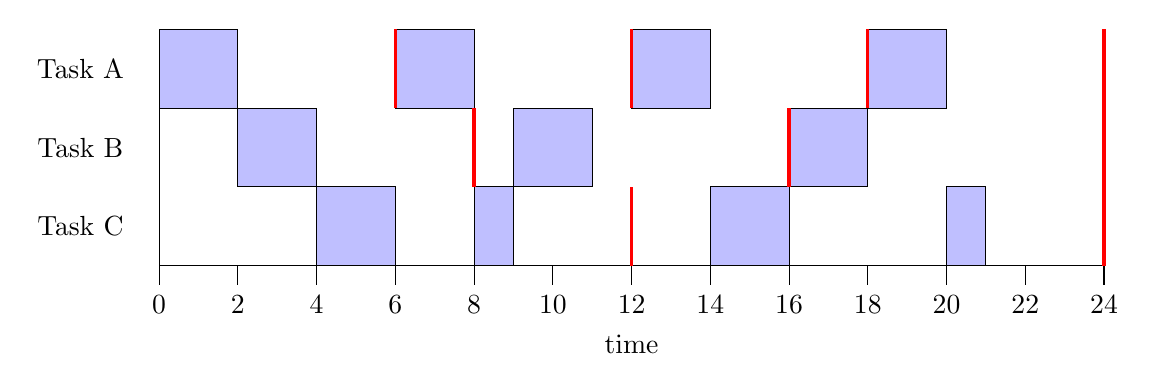
\begin{tikzpicture}[xscale=0.5]
                    \node at (-2,0.5) {Task C};
                    \node at (-2,1.5) {Task B};
                    \node at (-2,2.5) {Task A};
                    \node at (12,-1) {time};

                    \draw (0,0) -- (0,3);
                    \draw (0,0) -- (24,0);
                    
                    \pgfkeys{/pgf/number format/precision=0}

                    \foreach \i in {0,2,...,24} {
                        \draw (\i,0) -- (\i,-0.25);
                        \node at (\i,-0.5) {\i};
                    }

                    \draw[fill=blue!25!white] (0,2) rectangle (2,3);
                    \draw[fill=blue!25!white] (6,2) rectangle (8,3);
                    \draw[fill=blue!25!white] (12,2) rectangle (14,3);
                    \draw[fill=blue!25!white] (18,2) rectangle (20,3);

                    \draw[fill=blue!25!white] (2,1) rectangle (4,2);
                    \draw[fill=blue!25!white] (9,1) rectangle (11,2);
                    \draw[fill=blue!25!white] (16,1) rectangle (18,2);

                    \draw[fill=blue!25!white] (4,0) rectangle (6,1);
                    \draw[fill=blue!25!white] (8,0) rectangle (9,1);
                    \draw[fill=blue!25!white] (14,0) rectangle (16,1);
                    \draw[fill=blue!25!white] (20,0) rectangle (21,1);

                    \foreach \i in {6,12,...,24} {
                        \draw[deadline] (\i,2) -- (\i,3);
                    }

                    \foreach \i in {8,16,...,24} {
                        \draw[deadline] (\i,1) -- (\i,2);
                    }

                    \foreach \i in {12,24} {
                        \draw[deadline] (\i,0) -- (\i,1);
                    }
                    
                \end{tikzpicture}
            \end{center}

            Earliest Deadline First
            \begin{center}
                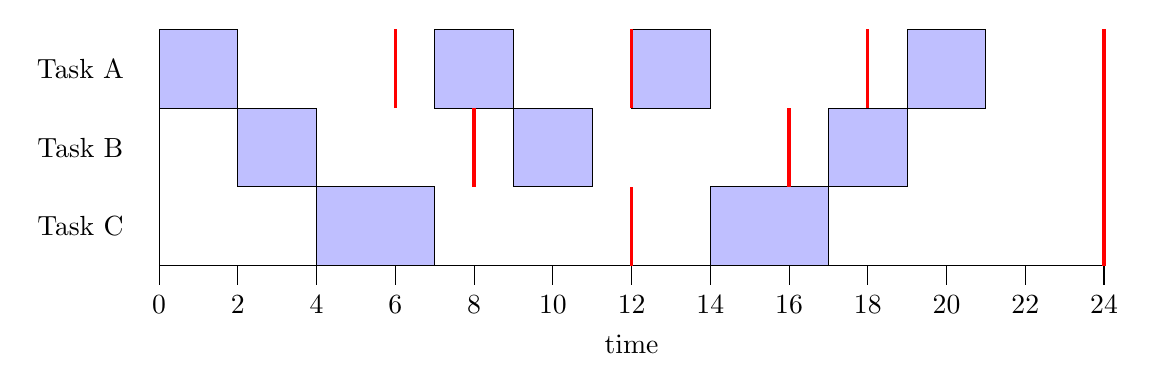
\begin{tikzpicture}[xscale=0.5]
                    \node at (-2,0.5) {Task C};
                    \node at (-2,1.5) {Task B};
                    \node at (-2,2.5) {Task A};
                    \node at (12,-1) {time};

                    \draw (0,0) -- (0,3);
                    \draw (0,0) -- (24,0);
                    
                    \pgfkeys{/pgf/number format/precision=0}

                    \foreach \i in {0,2,...,24} {
                        \draw (\i,0) -- (\i,-0.25);
                        \node at (\i,-0.5) {\i};
                    }

                    \draw[fill=blue!25!white] (0,2) rectangle (2,3);
                    \draw[fill=blue!25!white] (7,2) rectangle (9,3);
                    \draw[fill=blue!25!white] (12,2) rectangle (14,3);
                    \draw[fill=blue!25!white] (19,2) rectangle (21,3);

                    \draw[fill=blue!25!white] (2,1) rectangle (4,2);
                    \draw[fill=blue!25!white] (9,1) rectangle (11,2);
                    \draw[fill=blue!25!white] (17,1) rectangle (19,2);

                    \draw[fill=blue!25!white] (4,0) rectangle (7,1);
                    \draw[fill=blue!25!white] (14,0) rectangle (17,1);

                    \foreach \i in {6,12,...,24} {
                        \draw[deadline] (\i,2) -- (\i,3);
                    }

                    \foreach \i in {8,16,...,24} {
                        \draw[deadline] (\i,1) -- (\i,2);
                    }

                    \foreach \i in {12,24} {
                        \draw[deadline] (\i,0) -- (\i,1);
                    }
                    
                \end{tikzpicture}
            \end{center}

            Rate Monotonic Scheduling (priority is inverse to period)
            \begin{center}
                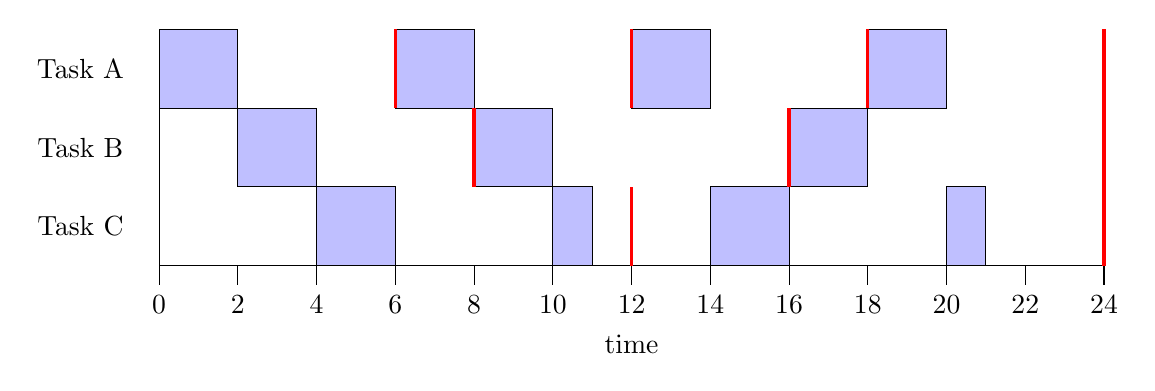
\begin{tikzpicture}[xscale=0.5]
                    \node at (-2,0.5) {Task C};
                    \node at (-2,1.5) {Task B};
                    \node at (-2,2.5) {Task A};
                    \node at (12,-1) {time};

                    \draw (0,0) -- (0,3);
                    \draw (0,0) -- (24,0);
                    
                    \pgfkeys{/pgf/number format/precision=0}

                    \foreach \i in {0,2,...,24} {
                        \draw (\i,0) -- (\i,-0.25);
                        \node at (\i,-0.5) {\i};
                    }

                    \draw[fill=blue!25!white] (0,2) rectangle (2,3);
                    \draw[fill=blue!25!white] (6,2) rectangle (8,3);
                    \draw[fill=blue!25!white] (12,2) rectangle (14,3);
                    \draw[fill=blue!25!white] (18,2) rectangle (20,3);

                    \draw[fill=blue!25!white] (2,1) rectangle (4,2);
                    \draw[fill=blue!25!white] (8,1) rectangle (10,2);
                    \draw[fill=blue!25!white] (16,1) rectangle (18,2);

                    \draw[fill=blue!25!white] (4,0) rectangle (6,1);
                    \draw[fill=blue!25!white] (10,0) rectangle (11,1);
                    \draw[fill=blue!25!white] (14,0) rectangle (16,1);
                    \draw[fill=blue!25!white] (20,0) rectangle (21,1);

                    \foreach \i in {6,12,...,24} {
                        \draw[deadline] (\i,2) -- (\i,3);
                    }

                    \foreach \i in {8,16,...,24} {
                        \draw[deadline] (\i,1) -- (\i,2);
                    }

                    \foreach \i in {12,24} {
                        \draw[deadline] (\i,0) -- (\i,1);
                    }
                    
                \end{tikzpicture}
            \end{center}
            
        \end{itemize}
    \end{itemize}

\end{document}